

\subsection{Преобразование Мёбиуса}
Преобразование Мёбиуса позволяет переводить коэффиценты из полинома Жегалкина в таблицу истинности и наоборот. 

\begin{center}
  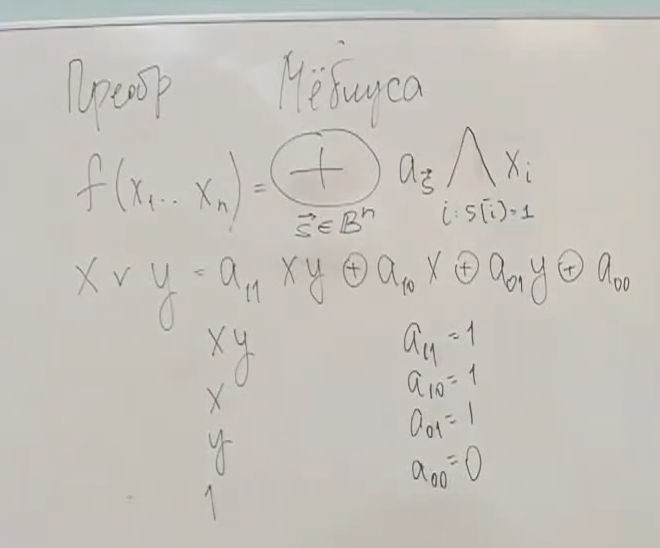
\includegraphics[height=9.1cm]{assets/Mebius.png}
\end{center}
  

Давайте заведем бинарные коэффиценты для полинома Жегалкина, которые будут отражать, берем мы или не берем то или иное слагаемое. Всего таких коэффицентов будет $2^n$, столько же, сколько и всего возможных членов полинома Жегалкина. Пронумеруем их так, если в члене нашего полинома есть $i$ый член, то в индексе коэффицента на $i$ом месте будет 1, иначе 0 (например для произведения $xz$ в полинома Жегалкина для функции от трех переменных индекс коэффицента будет 101). Получаем, что индекс коэффицента - булевый вектор какой-то длины, а его уже можно однозначто перевести в числовой коэффицент через двоичную систему счисления.
\newpage
Посмотрим на формулу с картиночки и начнем осознавать, откуда она взялась:
$\displaystyle f(x_1\dots x_n) = \bigoplus\limits_{\overrightarrow{s}\in\mathbb{B}^n}a_{\overrightarrow{s}}\bigwedge\limits_{i:s[i]=1}x_i$ - это просто формула полинома Жегалкина. Давайте разберемся, когда у нас $a_{\overrightarrow{s}}\bigwedge\limits_{i:s[i]=1}x_i=1$, очевидно это происходит, только в том, случае, если выполняется это: $\forall i : s[i] = 1, x_i = 1$. Назовем такое отношение \textbf{доминированием} и будем обозначать как $\leq$.
Тогда нашу формулу можно переписать как: $$\bigoplus\limits_{\overrightarrow{s}\in\mathbb{B}^n}a_{\overrightarrow{s}}\bigwedge\limits_{i:s[i]=1}x_i = \bigoplus\limits_{\overrightarrow{s}\leq \overrightarrow{x}} a_{\overrightarrow{s}}$$ 

Отлично у нас получилась формула перехода от одного базиса к другому, и, как и в линейной алгебре, ее можно записать с помощью матрицы перехода, независимо от того, какие функции у нас были. Например для четырех переменных она выглядит так:

\parbox{\textwidth}{
    \centering
    \begin{tabular}{ |c|c|c|c| }
        \hline
         1 & 0 & 0 & 0 \\
        \hline
         1 & 1 & 0 & 0 \\
        \hline
         1 & 0 & 1 & 0 \\
        \hline
         1 & 1 & 1 & 1 \\
        \hline
    \end{tabular}
}


При умножении данной таблицы на коэффиценты в полиноме Жегалкина, мы получим таблицу истинности, сейчас мы докажем, что при повторном умножении, мы обратно получим коэффиценты полинома Жегалкина, то есть докажем, что такая таблица обратна сама себе.

Давайте доказывать, хотим такую формулу: $$a_t=\bigoplus\limits_{x\leq t}f_x $$ Но мы уже знаем, что верно: $$\bigoplus\limits_{x\leq t}f_x = \bigoplus\limits_{x\leq t}\bigoplus\limits_{s\leq x}a_s=\bigoplus\limits_{x,s : s\leq x \leq t}a_s$$
Хорошо тогда давайте разберемся сколько раз мы взяли конкретный $s$. Если $t$ не доминирует над $s$, то очевидно 0. Иначе мы взяли $a_s$ 2 в степени количества битов $i$, таких что в $t[i]=1$ и $s[i]=0$. Очевидно что это число нечетное, только если их 0, то есть на самом деле $a_s$ влияет на сумму, только если $s=t$, а значит справа у нас изначально было написано $a_t$. \textit{QED}.

\subsection{Функциональные элементы}
Рассмотрим новый способ представления булевых схем - в виде ориентированного графа. Вершины в нем - это булевые значения, а ребра - операции с ними. 

$Глубина схемы$ - длина максимального пути между вершиной, названной входной и вершиной, названной выходной. 

\subsubsection{Топологическая сортировка}
\textbf{Топологическая сортировка} - такая сортировка вершин ориентированного графа, что если в ней вершина $u$ стоит раньше вершины $v$, то не сушествует ребра из $v$ в $u$.

\textbf{Теорема.} Топологическая сортировка существует, если в графе нет циклов и наоборот.

В левую сторону доказать совсем легко, если в графе есть цикл и топологическая сортировка в нем тоже существует, то мы можем найти самую правую вершину этого цикла в топологической сортировке и тогда ребро из нее будет вести влево, что противоречит определению топологической сортировки.

В правую сторону доказать немного сложнее, но все также нетрудно. Найдем вершину, из которой не ведет ни одного ребра в другие вершины, если такой нет, то цикл обязательно существует ведь мы можем запуститься из любой вершины и ходить по ребрам, пока не вернемся в уже посещенную вершину и получим цикл. Тогда удалим эту вершину, а в топологическую сортировку допишем ее слева, что не может сломать ее, ведь из этой вершины нет ни одного ребра в те, которые мы допишем позже. Продолжая этот алгоритм, мы и получим топологическую сортировку. 

